\documentclass[conference, 11pt]{IEEEtran}
\IEEEoverridecommandlockouts
% The preceding line is only needed to identify funding in the first footnote. If that is unneeded, please comment it out.
\usepackage{cite}
\usepackage{amsmath,amssymb,amsfonts}
\usepackage{algorithmic}
\usepackage{graphicx}
  \usepackage[utf8]{inputenc}
\usepackage{listings}
\usepackage{textcomp}
\usepackage{url}
%carltest Push
\usepackage{textcomp}
\def\BibTeX{{\rm B\kern-.05em{\sc i\kern-.025em b}\kern-.08em
    T\kern-.1667em\lower.7ex\hbox{E}\kern-.125emX}}
\begin{document}


\lstset{  	language=Python,
			basicstyle=\ttfamily,
			  columns=fullflexible,
			  frame=single,
			  breaklines=true}
			  
			  
\title{Connectivity Risk Analyzer: Development of an automated ETL Processs and investigation of AS-Level data\
{\footnotesize \textsuperscript{}}
\thanks{}
}

\author{\IEEEauthorblockN{Carl Tramburg}
\IEEEauthorblockA{\textit{M.Sc. Information Systems} \\
\textit{Humboldt University Berlin}\\
Berlin, Germany\\
carl.tramburg@gmail.com}
\and
\IEEEauthorblockN{David Berscheid}
\IEEEauthorblockA{\textit{M.Sc. Business Administration} \\
\textit{Humboldt University Berlin}\\
Berlin, Germany\\
d.berscheid@outlook.com}

}

\maketitle

%1. Introduction \\
%1A.  Motivation \\
%1B.  Evolution of CORIA \\
%1C.  Objectives \\
%
%2. Theoretical Background \\
%2A. Autonomous Systems \\
%2B. ETL \\
%
%3 Data \& (Framework) \\
%3A. Caida \\
%3B  (CORIA - ETL) \\
%
%4 Results \& Implementation \\
%4A Data Analysis (Crossectional Data) \\
%4B Data Analysis (Time Series) \\
%4C ETL Process  \\
%
%5 Conclusion \\
%5A Summary \\
%5B Limitations and Further Work \\

\begin{abstract}

Virtual networks are everywhere in todays digital world and cyber attacks are already part of daily news. With the ongoing cyber threats the need for IT security rises - and there is no recovery to be expected. Therefore, this paper poses further results of CORIA (Connetivity Risk Analyzer), a framework developed by Dr. Fabian and collegues to analyze multiple indicators explaining the risk of connections in a network like the internet - now introducing new features like an automated ETL process.

\end{abstract}

\begin{IEEEkeywords}
CORIA, Connectivity Risk Analyzer, ETL, Automation, AS, Autonomous System
\end{IEEEkeywords}


\section{Introduction}
\subsection{Motivation}
The internet presents one of the most important networks for today‘s world. Consequently major financial and economical systems rely on its functionality and availability. In times of non-functioning of the internet, serious consequences for businesses and economies are the result. There can be many reasons for such a scenario, such as threats caused by nature, i.e. hurricanes or earthquakes, or deliberate hacking attacks trying to remove nodes from the network.  
In 2016 for example the Dyn cyberattack, which involved multiple distributed denial-of-service attacks (DDos attacks) was the reason for large unavailability of internet platforms and services in North America and Europe. It is known as the larges DDoS attack on record, involving tens of millions of IP adresses\cite{dyn}. 900 000 users were infected by another attack in 2016, called Mirai Botnet, against the German company Deutsche Telekom, targeting routers and causing internet connectivity problems. \cite{DT}According to a study conducted by Ponemon Institute in 2016, the average cost of a data center outage has increased from \$ 505,502 in 2010 to \$ 740,357 in 2016\cite{Ponemon}. The list of cyber attacks could be much more extensive. Hacking is not the work of independent ideologists anymore but it can be assumed to be promoted and sponsored by large cooperations or governments manipulating and influencing events and relations all over the world \cite{cyberSponsors}, \cite{cyberSponsors2}, \cite{cyberSponsors3}. The implication on the importance of the internet becomes very clear, which gives high incentives to analyze the riskyness of these networks. CORIA's mission is exactely that: to help analyze connectivity risks\cite{Coria}.



\subsection{Evolution of CORIA}
The CORIA project started with the scope of a (master) thesis by Mathias Ehlert \cite{Ehlert}. With the objective of building a webframwork that is capable of analyzing connectivity risks of networks, CORIA 1.0 was developed. Through the access of large amount of network data, either publically available or individually provided, CORIA was able to calculate a variety of metrics, such as  
centrality measures or node degree measures, which then form a unified risk score for respective connectivity risks of respective nodes. In addition, CORIA offered a framework to investigate networks visually through graph visualisations. 
 The webapplication CORIA 1.0 was written in python and ruby. It used NetworkX for its metrics and redis for database purposes. After CORIA 1.5 presented a improved performance and the use of Graphtool instead of NetworkX for its metrics, Tom Kober developed CORIA 2.0 - now using Neo4j to store and manage data\cite{Coria1.5}. This version furthermore consisted of a native architecture of graph storage and processing\cite{Coria2}. CORIA 3.0 by Sebastian Gross benefits from modular based improvements. It offers different levels of granularity of networks that can be investigated.

 \begin{figure}[htbp]
\centerline{\includegraphics[scale=0.4]{Graphics/CORIAExtract.PNG}}
\caption{Extract of CORIA Dashboard}
\label{fig}
\end{figure}

 Figure 1 shows parts of the CORIA dashboard and figure 2 presents an example of a graph visualisation. Version 3 allows usage of all features via one interface. Due to the modular approach, there is a clear separation of ETL process, graph analysis and exports. Amongst its functionality is the usage of different data formats and the ability to calculate different metrics. The framework supports simultaneous execution and calculation of different metrics. Much attention was paid to a development without strong dependencies to specific technologies\cite{Coria3}.
   
..carl?... \\ 

 

\begin{figure}[htbp]
\centerline{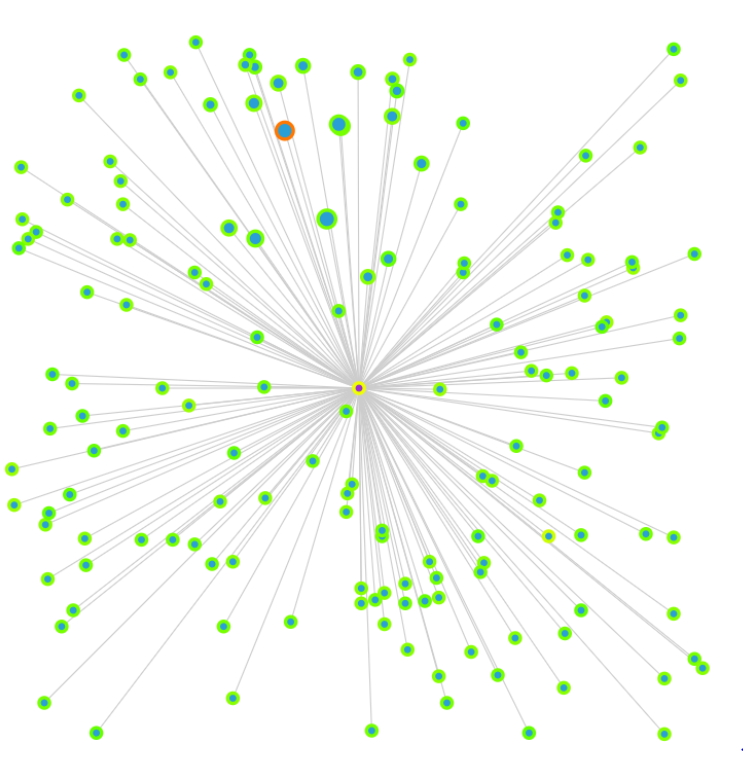
\includegraphics[scale=0.2]{Graphics/nodePresentaion.PNG}}
\caption{Graph Presentation of Nodes in a Network}
\label{fig}
\end{figure}



\subsection{Objective}
The CORIA framework is a project on which multiple developers already contributed to, in order to create a platform, which is able to analyze and visualize connectivity risks of graph data\cite{CoriaPaper}. Within this paper and project we would like to further contribute and improve specific aspects of CORIA. In the following we present related work regarding internet topology, the robustness of networks and characteristics of Autonomous Systems. We investigate characteristics of these networks through some descriptive statistical methods and take a look at the time development of networks and its components. Then we present an approach for an automated ETL process, which shall improve and simplify the usage of CORIA and ensure most recent data being available for analysis. Herby we focus on AS-level data. Our emphasis lies on flawless usage of datasets coming from the data source Caida that can be downloaded and imported automatically on a regular basis. \\



\section{Theoretical Background}
\subsection{Internet Topology}

The topology of the internet forms a clear hierarchy. As Figure 3 models it, on the lowest level of the internet topology are Internet Protocol network interfaces (IPs). Multiple Ips can access the internet through one router (R). Then, on the next level, Autonomous Systems (AS) represent a set of routers under a single administration. The top of this hierarchy is formed by Internet Service Providers (ISP), with selfdescribing funcionality. Note that this represents a simplified and high-level model of internet topology, i.e. not specifying Points of Presence \cite{ASH}. 

\begin{figure}[htbp]
\centerline{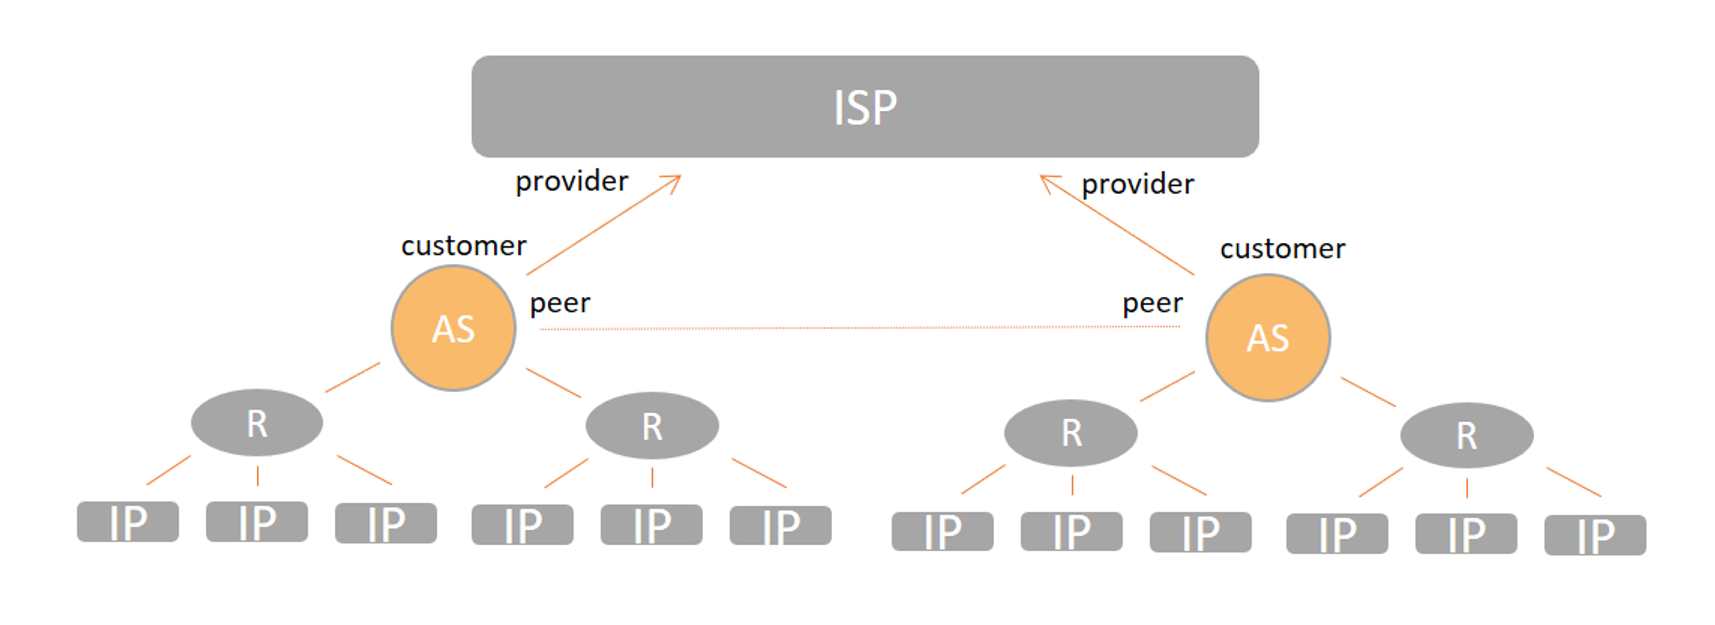
\includegraphics[scale=0.26]{Graphics/hierarchy.PNG}}
\caption{Hierarchy of the Internet}
\label{fig}
\end{figure}


 In the scope of this paper the level of Autonomous Systems is our main object of concern. Two types of relationships between ASes and ISPs are of interest in that regard: Provider-to-Customer (P2C) and Peer-to-Peer (P2P). \\



Figure 4 provides an example of an AS and its characteristics. Here Kabel Deutschland, a German network operator, represents an AS. Its customer cone specifies  ``a set of ASes it can reach using customer links''. As it is two in this case, there are only two nodes reached through customer links, meaning Kabel Deutschland itself and its provider Vodafone\cite{Rank}.  
%https://www.caida.org/~amogh/papers/asrank-IMC13.pdf
AS rank defines the importance of a node in its global routing system, often using customer cone information as a measure \cite{Rank}.
%http://as-rank.caida.org/about#goal
AS degree refers to the number of neighbors that a node has in a graph - here 20\cite{Cone}.  \\
\begin{figure}[htbp]
\centerline{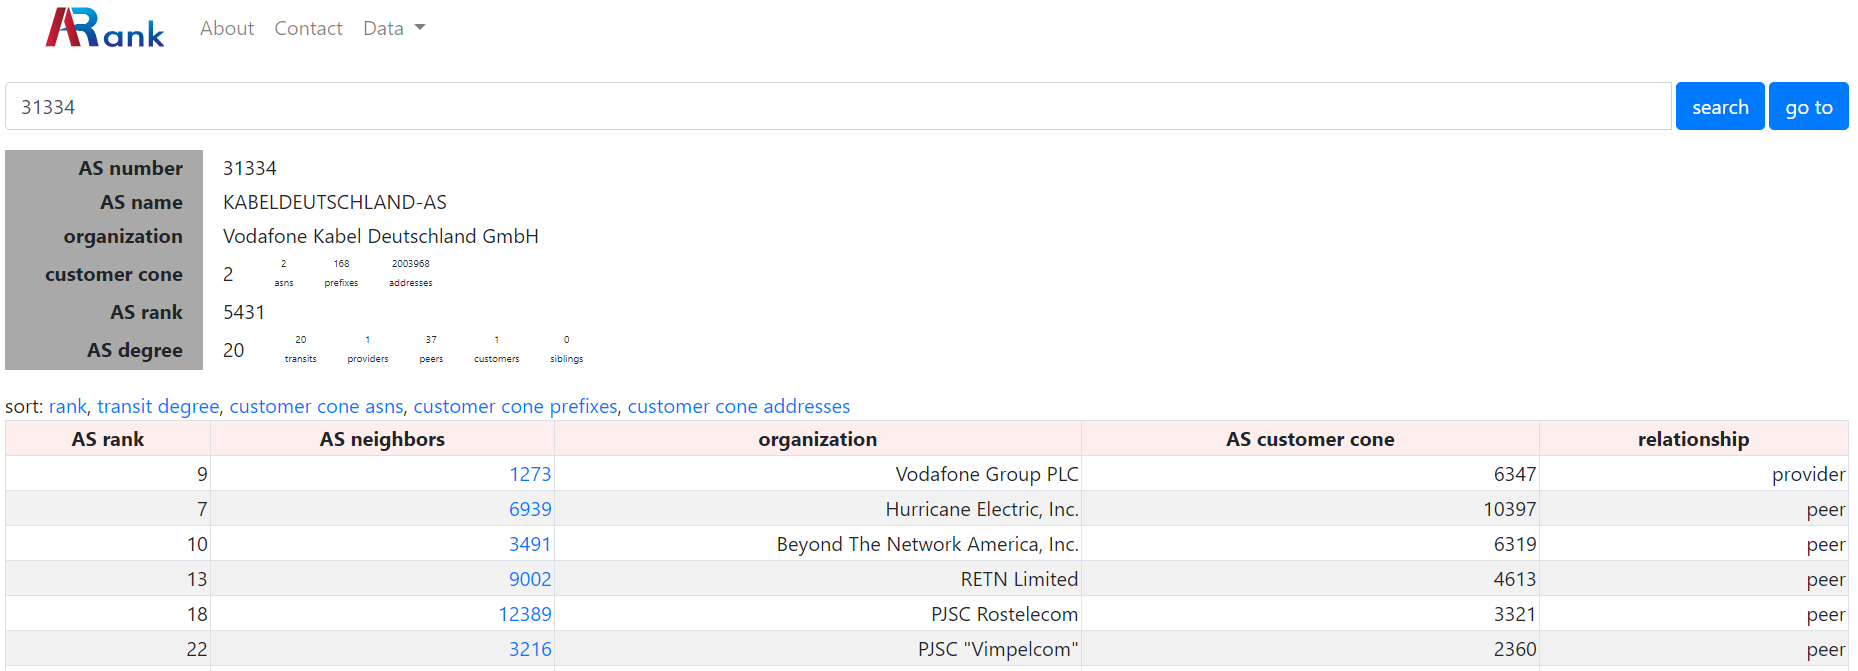
\includegraphics[scale=0.21]{Graphics/asExample.PNG}}
\caption{Example of an AS and its characteristics}
\label{fig}
\end{figure}




\subsection{Internet Robustness}
The internet is assabled based on the hierarchy as shown in figure 3. Much research has already been conducted on the robustness of the internet. 
Baumann and Fabian (\cite{howRobust}) state the following. While the internet is resistant with respect to random failures of nodes, a targeted atttack such as a degree attack can have a serious impact. The latter stands for an attack that focuses on the successive deletion of nodes with the highest node degree. They also pointed out that a targeted removal of only ten percent of the nodes of the network can lead to more than 32 000 disjoint components. Further research suggests that due to its evolution the internet network  is ``robust yet fragile''\cite{RYF}, meaning that random failures of nodes leave the network unaffected, whereas it is vulnerable to targeted attacks on its key components. Acoordingly, the internet is often reffered to as ``scale-free'' with a ``hub-like'' core structure, which leads to the described characteristics \cite{RYF}. Faloutsos et al. \cite{powerlawCitation} state in their research that the internet network is following a so called power-law distribution. Power-laws describe skewed distributions of graph properties, such as node degree. It can be used for estimating further characteristics of networks or an analysis of robustness. Note though that they base their research on data from November 1997 and December 1998. J. Ruiz and G. Barnett also make statement about the imbalancedness of the internet \cite{owningInternet}. Their results indicate that the United States is the most central nation in the network, with American corporations accounting for almost 40\% of international links between nodes. Moreover they state that there exists a center of the network consisting of 16 companies, each causing more than 1\% of international internet connections.  
Research of \cite{geoResearch} in 2002 modeled the internet's large scale topology - amongst others the geographic locations of routers. In that regard, they published the geographic locations of routers and found a major concentration in North America and Europe and muss less activity on other, less developed continents.\\ 
 


\subsection{ETL Process}
The data warehousing concept of \textit{Extraction, Transformation, Loading} (ETL) became a standard for companies in the 1970s. Back then organizations began to integrate information from different sources into their own databases \cite{carl1}.\break The integration process states the advantage that disparate sources and hereby diverse formation of the data can be brought into a unified database. With an adjustable ETL process one is able to adapt to and import new datasources without 
changing the essential main system or framework. This segregation of data import and processing makes the whole system more stable, flexible, provides improved maintance and makes it easier for developers to change and extend functionalities. %Quelle 

\begin{lstlisting}
import networkx as nx

G=nx.complete_graph(20)
nx.write_edgelist(G, "test3.edgelist", delimiter="\t", data=False)
H=nx.complete_graph(100)
nx.write_edgelist(G, "test2.edgelist", delimiter="\t", data=False)

quit()
\end{lstlisting}

\break
\break
\break

\begin{figure}[htbp]
\centerline{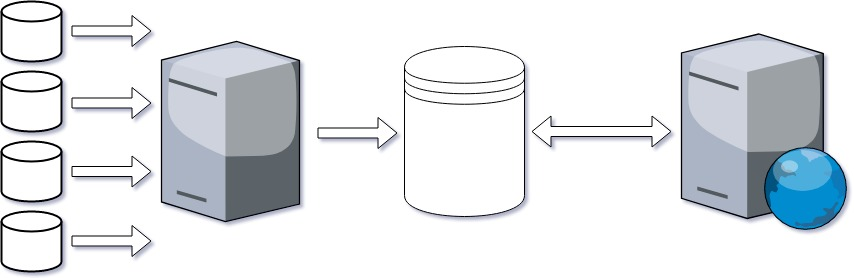
\includegraphics[scale=0.27]{Graphics/ETL_general.png}}
\caption{Visualization of a general ETL process}
\label{fig1_ct}
\end{figure}


A general ETL workflow is presented in figure \ref{fig1_ct}.  
\iffalse

extraction:
- different souces, format, files, interfaces (ftp, api, js-call)
-import to server

Transformation:
- eradicate differences, calculations, analysis, create unified dataformat

Load:
- upload to database,
- p.ex. organization: different departements different insights -> combined T+L ->to fulfill orgas compliance or segragation of duty need to know principles - relevance in data security and information governance.

#####
The current caida etl process will be presented in ref X
and our contribution is described in ref Y






Carls part, blablabalhalohaloo \\ 

Extraction: from data source(s), varying data formats
Transform: convert different data into proper format, that is storable

Load: load into target database

\fi



\begin{figure}[htbp]
\centerline{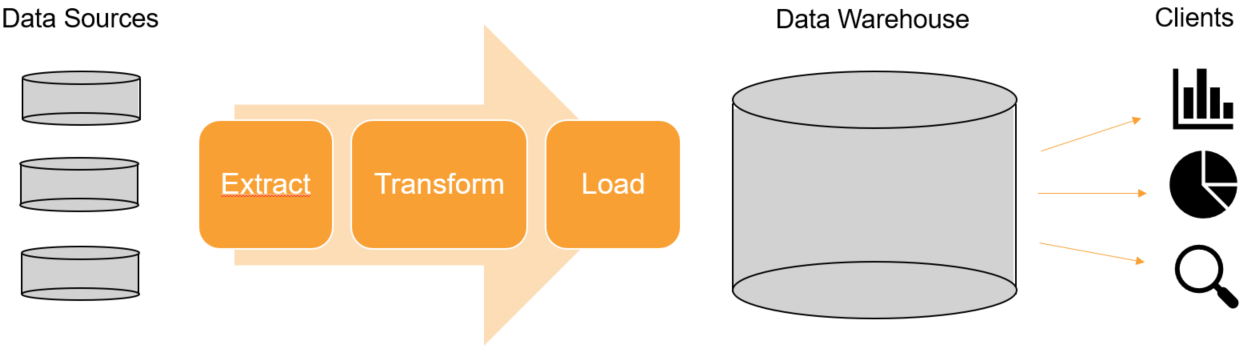
\includegraphics[scale=0.3]{Graphics/ETLTheory.PNG}}
\caption{Theoretical ETL Process}
\label{fig}
\end{figure}




\subsection{Data Science, BI, Software Engineering, Design Science Research} 



\section{Data}
As a data source for this work, we exclusively focus on Caida. Caida is an appreviation and stands for Center for Applied Internet Data Analysis. Located in San Diego, CA in the United States, the center studies networks and its infrastructure up to a large scale. For their investigation on theoretical and practical aspects of the internet they monitor, collect and provide network data \cite{Caida}. 

Regarding the data granularity our primary focus lies on AS level data. Within this domain, we investigate five type of datasets. \textit{AS-Rank} offers a data base giving information about specific Autonomous Systems, like its rank, relationship to other ASes or customer cone  \cite{Rank} . \textit{AS Classification} represents a dataset including information on the business types of Autonomous Systems \cite{Classification}. Through machine-learning inference, Caida is able to offer this knowledge  \cite{Classification}. A large collection of datasets named \textit{Pv4 Routed 24 AS Links} is used in detail to investigate the topology on the internet, its structure regarding streams of traffic, and ratios of sending and receiving autonomous systems  \cite{IPv4Data}. This collection of data forms the center of our investigation. From 2007 to 2018 data is collected, by three \textit{teams}. Caida uses independent teams to collect data in order to offer a way to validate the data and its data inference. The teams probe every routed /24 in the IPv4 address space.
We investigate the dataset \textit{AS Relationships} in order to find out about Provider to Customer relationships as well as Peer to Peer relationships \cite{CaidaRelationshipsData}.  Lastly, we take into account geographic information of the Autonomous Systems to draw conlclusions on regions with high imapact on the internet network and less involved ones  \cite{CaidaGeoData}. 


For the purpose of investigating the characteristics of Ases itself and their network, we analyzed recent data of December 2017.  As for the time series analysis, we used data from 2007 until 2017. \\

how many nodes? observations? lines of code?

\section{Results}

\subsection{Data Analysis}
First aspect of the data analysis process is the type of autonomous system. Caida distinguished here between three types: The first type are ASes that provide internet access or function as a transit. They make out 42.2\% of all nodes in the network. Second type are ASes providing content hosting and distribution systems, like Dropbox or Google, with only 4,5\% of all overall nodes. Third category are enterprises meaning organizations, universities or companies that are mostly users. They account for 53.3\%. Insights we are gaining from this aspect is that most of the nodes are representing users of the internet, which makes intuetively sense. More interesting is the large amount of transits and access points needed to provide the respective infrastructure. This hints to the internet's high complexity. 


\begin{figure}[htbp]
\centerline{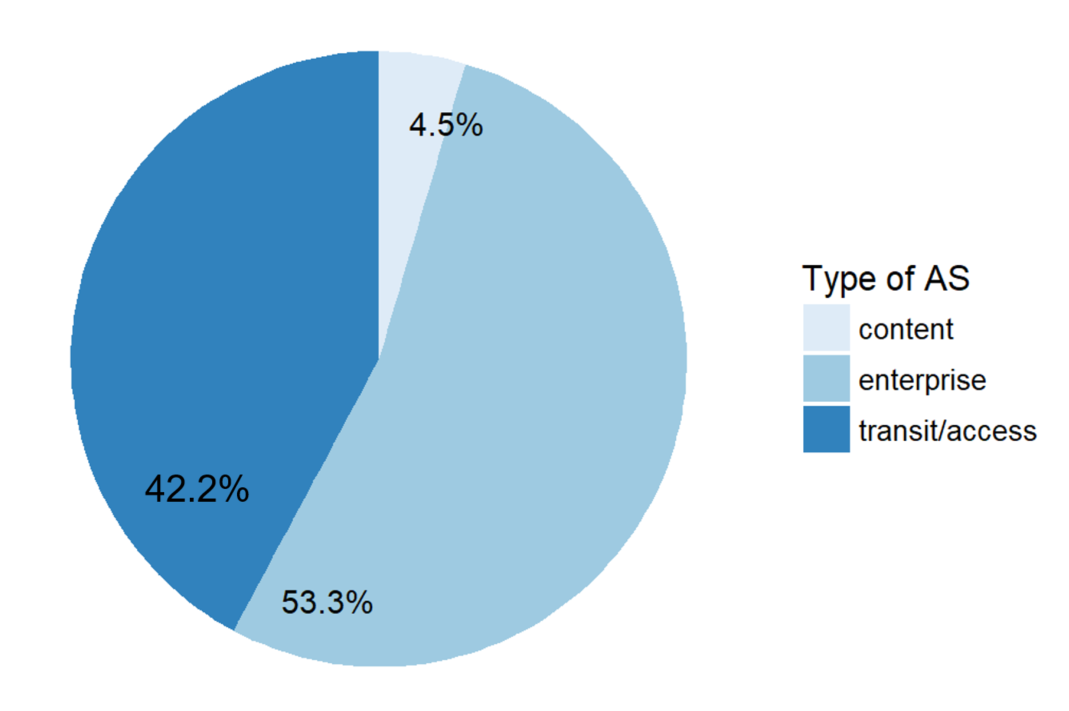
\includegraphics[scale=0.4]{Graphics/typeofAS.PNG}}
\caption{Ratio of Autonomous Systems regarding their Type }
\label{fig}
\end{figure}

As depicted in the theoretical part, autonomous systems have relationships. We took a look at this characteristic in figure 7 and noticed quite a balanced ratio of Provider-to-Customer relations and Peer-to-Peer relations. If we translate this into a graph, we imagine a balanced graph, which in terms of network riskiness, is rather roboust. 

\begin{figure}[htbp]
\centerline{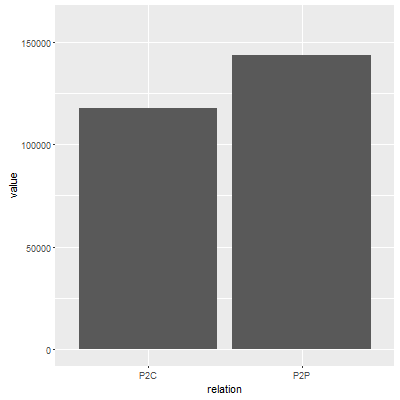
\includegraphics[scale=0.45]{Graphics/relationspeerandprovider.png}}
\caption{Ratio of AS-Relationships }
\label{fig}
\end{figure}


We furthermore built graphs describing the distributional characteristics of autonomous systems. Figure 8 shows the distribution of autonomous systems and how many outgoing connections the single nodes have. Approximately 5.500 sending nodes are containted within that data set. We ranked them on the x-axis. With the number of connections an AS is sending to on the y-axis, we obtrain a very left centered distribution. A very small number of nodes in the network are sending traffic to a high number of other nodes. It follows, what is called a power-law distribution  \cite{powerlawCitation}. Calculating the quantiles of the distribution, the top 10 percent of highest ranked nodes (ranked by the number of different outgoing connections) send to almost exactely 50\% of overall trafic of the whole network. The top five percent are responsible for 36\% of all outgoing traffic and the top one percent even accounts for approximately 17\%. Note that when we make statements of the whole network, we only refer to the data at hand as the whole network. That is the data collected by CAIDA. Information on CAIDA's data collection process can be found in \cite{CaidaDataCollection} . 

%> sum(sumAsTo$count[1:4900]) / sum(sumAsTo$count)
%[1] 0.5059264
%> sum(sumAsTo$count[1:2450]) / sum(sumAsTo$count)
%[1] 0.3608107
%> sum(sumAsTo$count[1:490]) / sum(sumAsTo$count)
%[1] 0.1678801

Simultaneousely, we drew the distribution of incomming connections per Autonomous System (Appendix ...) and received a similar result. With approximately 250.000 nodes, receiving traffic, only very few nodes are receiving traffic from a high number of nodes, again following the properties of a power-law distribution. The top ten percent of highest ranked nodes, are receiving approximately 52\% of the overall trafic in this network. The top five percent make up 36\% and the top one percent even 17\% of overall trafic. The quantiles are almost identical to those of the previous distribution. 

%top 1 percent
%> sum(sumAsTo$count[1:520]) / sum(sumAsTo$count)
%[1] 0.1724906


%top 5 percent
%2500 / 52055  = 0.05
%> sum(sumAsTo$count[1:2500]) / sum(sumAsTo$count)
%[1] 0.3646528
 

% 10 percent
%> sum(sumAsTo$count[1:5200]) / sum(sumAsTo$count)
%[1] 0.5174527

An important finding regarding connectivity risks of the network is, how vulnerable this network is. An attack targeting the most active and most influential nodes in the network, achieving a non-functioning of those quickly leads to wide shot-downs of the network. Previous introduced results by \cite{powerlawCitation} and \cite{owningInternet} can therefore be supported.  This again underscores the demand for CORIA - a tool to analyze connectivity risks. 


\begin{figure}[htbp]
\centerline{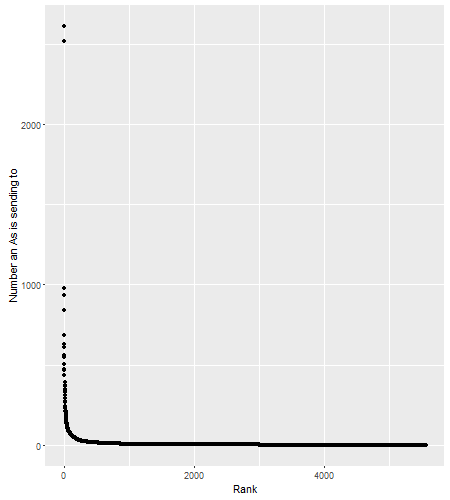
\includegraphics[scale=0.4]{Graphics/AsFromDistribution.png}}
\caption{Distribution of Outgoing Connections per AS}
\label{fig}
\end{figure}



Next, we analyzed the geographic locations of autonomous systems and their flow of traffic. Figure 9 symbolizes autonomous systems as organge points on a word map. We can see a high concentration of ASes in North America and Europe. The concentration of ASes is less dense in areas like South America, Africa or Asia. Insights that we can draw from that representaion are that more autonomous systems are situated in highly developed economies  than they are in less developed regions. This result corresponds to previous research conducted by \cite{ResearchGeo}. While we need to keep in mind that we are only analyzing one data set - with challenging data collection on top of that, we can assume this result still to be a representative sample of the overall network \cite{CaidaDataCollection}. The results confirm the assumption that most traffic is taking place between parties of richer and more developed economies.  (auf punkte ohne verbindung hinweisen?)
These results confirm the research from 2002 by \cite{geoResearch} and lead to the conclusion that the geographically speaking the internet network did not develop much further. Accordingly, one can state that developed areas increased their power and wealth, whereas in the last 15 years the development of less wealthy areas is only marginal. Even though we are looking at the level of Autonomous Systems and \cite{geoResearch} looked directly at the router-level, the comparison remains valid. \\



\begin{figure}[htbp]
\centerline{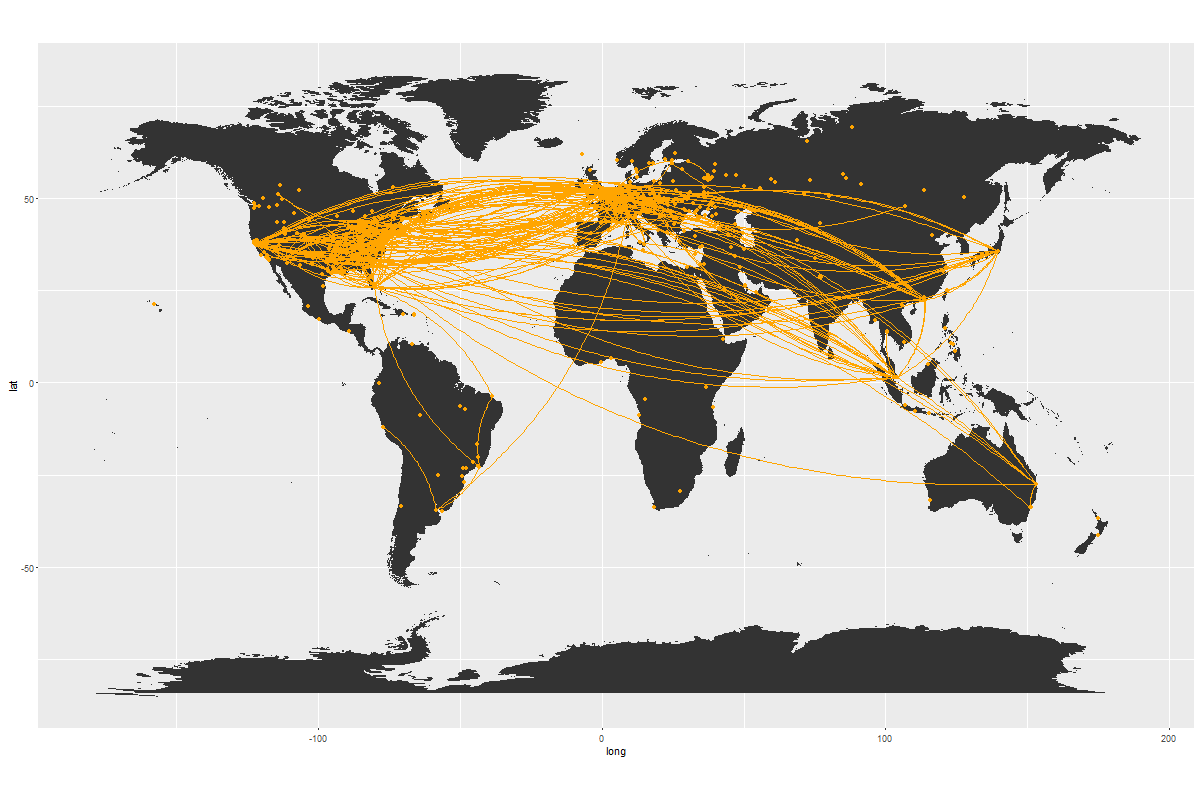
\includegraphics[scale=0.2]{Graphics/connectedASes.png}}
\caption{Location of ASes and respective Streams of Traffic}
\label{fig}
\end{figure}

In addition to the analysis of a single point in time, we investigated the timely development of the network. Figure 10 shows the number of traffic-sending autonomous systems from the beginning of 2007 until the end of 2017. Within these 10 years, there is a clear upward trend. In 2015 this upward trend vanishes and and reaches a constant level of approximately 5.500 sending AS nodes within the network. (Note the consistency of results with respect to  the `Distribution of number of sending ASes` in the appendix) Striking in that graph are the multiple outliers appearing throught the time series. A qualitative research about exeptional events happening on these dates that might have been the reason for a downtime of multiple nodes did not lead to reasonable results. As a consequence, we assume the outliers to be caused by monitoring and data collection problems of CAIDA \cite{CaidaDataCollection}

With respect to Appendix .....  you can see a simultaneous development for the amount of nodes, receiving traffic - on a level of approx. 250.000 nodes of course. 


\begin{figure}[htbp]
\centerline{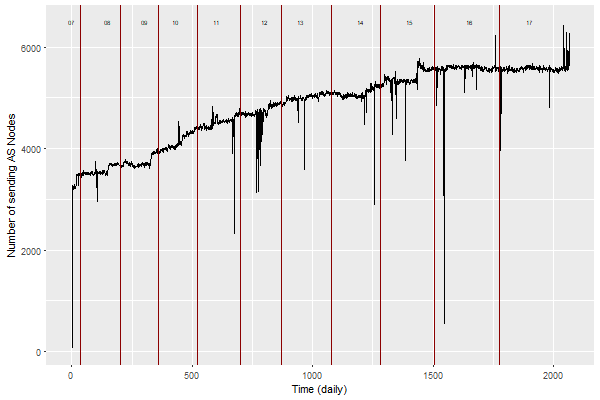
\includegraphics[scale=0.4]{Graphics/ASFromAll.png}}
\caption{Time development from 2007 - 2017: Number of sending AS nodes}
\label{fig}
\end{figure}


\subsection{ETL Process in CORIAv3}
The seminar paper is based on the framework of Sebastian Gross\cite{carl3}. At the current state CORIA does not include any automated ETL process for any source. The extraction part is handled manually by downloading the desired files and, if neccessary, unzipping the text-formatted file that for instance can be an edge list. \linebreak


The user can now upload the file using the CORIA web interface. This must be done with the upload module (\url{http://localhost:8080/coria/#!/datasets/upload}).
The upload module itself already provides Caida specific upload functions that can handle Caida's file format\cite{carl3}. As well a "Standard tab seperated Importer" allows users to upload edge lists from other sources. At the moment Coria only accepts edge lists of undirected unweightes graphs.
Users must be able to adjust or transform data into the demanded format. The current transformation part in the framework consists in transformation that has to be done by the user.\linebreak


After manually preprocessing the dataset, the web framework allows the user to upload the edge list and then analyze and apply metrics to the data.
Coria already provides modules that can upload data into a MySQL or Redis database. Unexperienced users do not need to be familiar with database management systems.








\begin{figure}[htbp]
\centerline{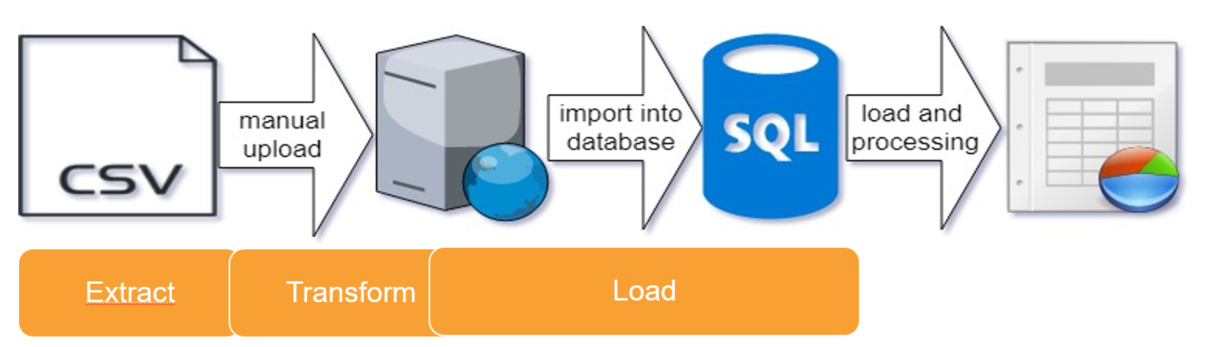
\includegraphics[scale=0.29]{Graphics/ETL1.PNG}}
\caption{A Theoretical ETL Process}
\label{fig}
\end{figure}



\begin{figure}[htbp]
\centerline{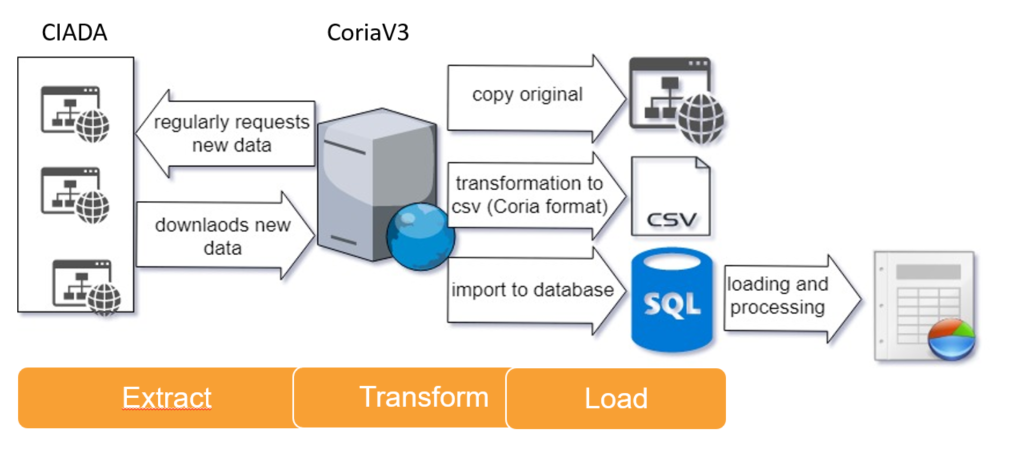
\includegraphics[scale=0.4]{Graphics/ETL2.PNG}}
\caption{ETL Process in the Coria framework}
\label{fig:1}
\end{figure}

In figure \ref{fig:1} the automated ETL process from Caida's data is illustrated. The framework is written in Python 2.7 %Python Software Foundation. Python Language Reference, version 2.7. Available at http://www.python.org

In general:Tthe server periodically queries for new data sets on the Cadia data server. If there are not new data uploaded on the Caida server the query will happen the next period. 
For the case new data are provided every new file will be downloaded. After downloading a new file, it will be transformed into an edgelist and ,finally, uploaded to Coria's database.
\linebreak
\linebreak

*For Caida data a daily iteration of the queries is sufficient as uploads are made every week on average - But as we can see from figure(upload histogram 2016 - 2018) a vast variation on the upload data and amount of files 

*at the End tell for the case of 1st time implementation and time on server
In detail:

Ensuring that the automated ETL process and all of its function trigger every day, we created a function \textit{timer.py}?REF. The timer program is meant to operate permanently after Coria webservice and the MySQL database are functioning.
An 24 hour interval is deemed to be adequate as Caida's data file provides AS link snapshot of one day. Besides that Caida teams upload their data unsystematically: As we can observe in figure \ref{figure Histogram of uplaod} there at some days with more than 20 uploaded files(data days). As well long there are periods in summer and around new years eve with none or a few uploads that can be assumed as holidays.
For other sources or data sets the interval can be customized by changing the sleep timer values of seconds.

%The timer program also makes use of \{syntax errors and exceptions} %ref https://docs.python.org/2.7/tutorial/errors.html#exceptions
From our coding experience infinite Python loops could create unsystematiclly errors.





\begin{figure}[htbp]
\centerline{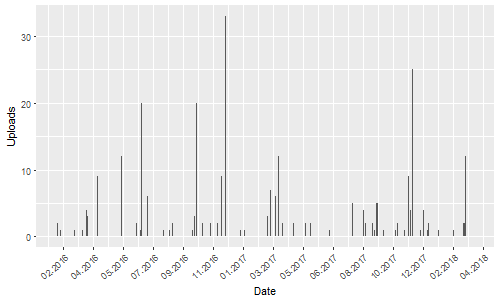
\includegraphics[scale=0.5]{Graphics/uploadFrequency.png}}
\caption{Data Uploads by Caida over time}
\label{fig}
\end{figure}



\section{Conclusion}
\subsection{Summary}

The webapplication CORIA allows the analysis of connectivity risks of various network graphs. Through visualizations and a unified risk score it offers comprehensive results. Fokussing on the level of Autonomous Systems, our data analysis revealed a power-law distribution when it comes to the influence of ASes within the internet network - a few highly important nodes and many less important ones. Moreover the geographical investigation of its locations showed the high concentration and flow of traffic of ASes in highly developed economies, with only sparse density in less developed economies. With regard to the trend of the internet network, we exhibited a linearly growing trend of AS nodes until 2015, when the size of the network stayed constant until today.

Regarding the software-development aspect, we developed an ETL tool in Python that provides automation of the validation of latest data files, copying respective files, and transforming them into csv format.  (haben wir noch mehr gemacht?)

 

\subsection{Limitations and Further Work}

 
One limitation of this work is caused by our data source Caida. The data that we used, i.e. types of Autonomous Systems or their relationship was partly gathered through statistical inference. Its machine learning classifier provided a positive predicted value of 70\% \cite{Classification}, which still leaves misslassified observations within the data and limits our results to some extent. Nevertheless Caida is a serious and trusted source, which is why we chose it in the first place. To our best knowledge, there is no superior data souce available.  \\ 

other limitations\\



Further work that can follow could be to apply the automated ETL process to further data sources, than only Caida. Also, deploying the the CORIA framework on a server would be a neccessary improvement. (CARL? Was hat es mit diesem Punkt auf sich? Läuft es nicht schon auf einem Server?) For improvements of internal development activities the creation of an extensive code and installation documentation is helpful.



\begin{thebibliography}{00}


\bibitem{dyn}K. York. (2016, Oct.) Dyn’s Statement on the 10/21/2016 DNS DDoS Attack, [Online]. Available: https://dyn.com/blog/dyn-statement-on-10212016-ddos-attack/
\bibitem{DT}E.Auchard. (2016, Nov.)Deutsche Telekom attack part of global campaign on routers, [Online]. Available: https://www.reuters.com/article/us-deutsche-telekom-outages/deutsche-telekom-attack-part-of-global-campaign-on-routers-idUSKBN13O0X4
\bibitem{Ponemon}Ponemon Institute LLC, ``Cost of Data Center Outages,'' Data Center Performance Benchmark Series, 2016 %https://www.vertivco.com/globalassets/documents/reports/2016-cost-of-data-center-outages-11-11_51190_1.pdf


\bibitem{cyberSponsors} By EWEN MACASKILL and GABRIEL DANCE Produced by FEILDING CAGE and GREG CHEN Published on November 1, 2013. Available: https://www.theguardian.com/world/interactive/2013/nov/01/snowden-nsa-files-surveillance-revelations-decoded.
\bibitem{cyberSponsors2}R.Barton, ``Chinese cyberattack hits Canada's National Research Council,'' CBC News. Available: http://www.cbc.ca/news/politics/chinese-cyberattack-hits-canada-s-national-research-council-1.2721241
\bibitem{cyberSponsors3}A.Kharpal, ``North Korea government-backed hackers are trying to steal cryptocurrency from South Korean users,'' CNBC, Available: https://www.cnbc.com/2018/01/17/north-korea-hackers-linked-to-cryptocurrency-cyberattack-on-south-korea.html



\bibitem{Coria}B. Fabian et al., `` CORIA – Analyzing Internet Connectivity Risks Using Network Graphs,'' IEEE International Conference on Communications Paris (IEEE ICC 2017), May 2017. 10.1109/ICC.2017.7996828. 
\bibitem{Ehlert}M. C. Ehlert, "A Software Framework for Analyzing Connectivity Risk of Graph Data," Master of Science, Humboldt-Universität zu Berlin, 2014. 
%\bibitem{Coria1} fehlt noch
%\bibitem{Coria1.5} fehlt noch 
\bibitem{Coria2} D.Kiene-Maksimovic, E. Zinovyeva, J. Park, ``CORIA 2.0: Augmenting a Universal Framework for Connectivity Risk Analysis,'' Jahr???
\bibitem{Coria3}S.Gross, ``Entwicklung eines modularen Frameworks für die Analyse von Verbindungsrisiken von Netzwerken basierend auf Netzwerkgraphen,'' November 2017.
\bibitem{CoriaPaper}
\bibitem{ASH}
 \bibitem{Rank}Caida., ``AS Rank,'' [Online]. Available: http://as-rank.caida.org/.
\bibitem{Cone}M. Luckie et al., "AS Relationships, Customer Cones, and Validation", Internet Measurement Conference (IMC), Oct 2013, pp. 243--256.
\bibitem{howRobust}Baumann, A., Fabian, B. 2015. “How Robust is the Internet? – Insights
from Graph Analysis,” in Proceedings of the 9th International
Conference on Risks and Security of Internet and Systems (CRiSIS
2014), Trento, Italy, Springer, LNCS 8924, pp. 247-254.
\bibitem{RYF}Albert, R. Jeong, H. and Barabasi, A.-L. (2000) Nature 406, 378–382.
 \bibitem{powerlawCitation}M. Faloutsos, P. Faloutsos, and C. Faloutsos, “On power-law relationships of the Internet topology,” Proc. of ACM SIGCOMM ’99, Cambridge, MA, Aug. 1999, pp. 251–262.
\bibitem{owningInternet}J. Ruiz, G. Barnett, ``Who owns the international Internet networks?,'' The Journal of International
Communication. November 2014. 21:1, 38-57, DOI:
10.1080/13216597.2014.976583
\bibitem{geoResearch}S. Yook, H. Jeong, A. Barabasi, ``Modeling the Internet's Large-Scale Topology, '' Proceedings of the National Academy of Sciences of the 
United States of America, November 2002.

\bibitem{carl1}SAS Institute GmbH (n.d.). Retrieved from \url{https://www.sas.com/en_us/insights/data-management/what-is-etl.html}



\bibitem{Caida}Caida, [Online] Available: https://www.caida.org/home.
\bibitem{Classification}Caida., ``AS Classification,'' [Online]. Available: http://www.caida.org/data/as-
classification.
\bibitem{IPv4Data}Caida., ``IPv4 Routed /24 AS Links Dataset,'' [Online]. Available: http://www.caida.org/data/active/ipv4\_routed\_topology\_aslinks\_dataset.xml.
\bibitem{CaidaRelationshipsData}Caida., ``AS Relationships,'' [Online]. Available:http://www.caida.org/data/as-relationships/.
\bibitem{CaidaGeoData}Caida., ``AS Relationships -- with geographic annotations,'' [Online]. Available: http://www.caida.org/data/as-relationships-geo/.
\bibitem{CaidaDataCollection} 


%aus unserer Präsi:

%B. Fabian, G. Tilch, “Analyzing the Global-Scale Internet Graph at Different Topology Levels: Data Collection and Integration“.
%D. Kiene-Maksimivic, E. Zinovyeva, J. Park, “CORIA 2.0: Augmenting a Universal Framework for Connectivity Risk Analysis”, 2017.
%J. Dümig, “Modelling of an Extraction Transformation Loading (ETL) system for the connectivity risk analyzing framework CoRiA“, 2016.
%M. Luckie et al., “AS Relationships, Customer Cones, and Validation”, Internet Measurement Conference, 2013.
%M. Oehlers, B. Fabian, ”Graph Metrics for Internet Robustness: A Survey”, ACM Comput. Surv. 1, 1, Article 1, 2018.
%S.Gross, “Development of a modular software framework for the analysis of network connectivity risks based on network graphs”, 2017.
%T. Kober, “Business Intelligence in der Telekommunikation : Konzeption und Umsetzung einer Graphendatenbank mittels Neo4j“, 2016.

%ende aus unserer präsi

 

\bibitem{powerLaw} Yaneer Bar-Yam. ``Concepts: Power Law," New England Complex Systems Institute, August 2015.
\bibitem{CaidaRelationships}X. Dimitropoulos, G. Riley, ``Modeling Autonomous System Relationships,'' Principles of Advanced and Distributed Simulation (PADS), May 2006, pp. 143--149.
\bibitem{RelInference}X. Dimitropoulos et al., ``Revealing the Autonomous System Taxonomy: The Machine Learning Approach," Passive and Active Network Measurement Workshop (PAM), Mar 2006.
\bibitem{CaidaRel2}X. Dimitropoulos et al., "Classifying the Types of Autonomous Systems in the Internet", SIGCOMM, Aug 2005.
\bibitem{ResearchGeo}







\bibitem{graphMetrics}M. Oehlers, B. Fabian, ``Graph Metrics for Internet Robustness: A Survey,'' ACM Comput. Surv. 1,1, Article 1, January 2018.
\bibitem{BAETL}J.Dümig, ``Modelling of an Extraction Transformation Loading (ETL) system for the connectivity risk analyzing framework CoRiA, December 2016.
\bibitem{BA}T.Kober, ``Business Intelligence in der Telekommunikation: Konzeption und Umsetzung einer Graphendatenbank mittels Neo4j,'' December 2016.

\bibitem{carl2}butunclebob(n.d.). Retrived from \url{http://butunclebob.com/ArticleS.UncleBob.PrinciplesOfOod}

\bibitem{carl3} S. Gross "Development of a modular software framework for the analysis of network
connectivity risks based on network graphs" (Bachelor thesis), 2017

%mehr Quellen von Prof Fabian:
\bibitem{geoVul}A. Baumann, B. Fabian. ``Towards Measuring the Geographic and Political Resilience of the Internet,'' International Journal of Networking and Virtual Organisations, 13(4):365–384, 2013.

%Damien Magoni. Tearing Down the Internet. IEEE Journal of Selected Areas in Communications, 21(6):949–960, September 2006.


%Martin Huth and Benjamin Fabian. Inferring Business Relationships in the Internet Backbone. International Journal of Networking and Virtual Organisations, 16(4), 2016.


%Annika Baumann and Benjamin Fabian. Who Runs the Internet? Classifying Autonomous Systems into Industries. In Proceedings of the 10th International Conference on Web Information Systems and Technologies (WEBIST), Barcelona, Spain, 2014.

%Annika Baumann and Benjamin Fabian. Vulnerability Against Internet Disruptions – A Graph-based Perspective. In Proceedings of the 10th International Conference on Critical Information Infrastructures Security (CRITIS 2015), Berlin, Germany, LNCS, Vol. 9578, Springer, 2015.


%Benjamin Fabian, Annika Baumann, and Jessica Lackner. Topological Analysis of Cloud Service Connectivity. Computers & Industrial Engineering, 88:151–165, 2015






abstand\\
%die quellen sind nur als Formatvorlage gedacht:
%\bibitem{b1}still old!noch die aus der Präsi einfügen'! G. Eason, B. Noble, and I. N. Sneddon, ``On certain integrals of Lipschitz-Hankel type involving products of Bessel functions,'' Phil. Trans. Roy. Soc. London, vol. A247, pp. 529--551, April 1955.
%\bibitem{b2} J. Clerk Maxwell, A Treatise on Electricity and Magnetism, 3rd ed., vol. 2. Oxford: Clarendon, 1892, pp.68--73.
%\bibitem{b3} I. S. Jacobs and C. P. Bean, ``Fine particles, thin films and exchange anisotropy,'' in Magnetism, vol. III, G. T. Rado and H. Suhl, Eds. New York: Academic, 1963, pp. 271--350.
%\bibitem{b4} K. Elissa, ``Title of paper if known,'' unpublished.
%\bibitem{b5} R. Nicole, ``Title of paper with only first word capitalized,'' J. Name Stand. Abbrev., in press.
%\bibitem{b6} Y. Yorozu, M. Hirano, K. Oka, and Y. Tagawa, ``Electron spectroscopy studies on magneto-optical media and plastic substrate interface,'' IEEE Transl. J. Magn. Japan, vol. 2, pp. 740--741, August 1987 [Digests 9th Annual Conf. Magnetics Japan, p. 301, 1982].
%\bibitem{b7} M. Young, The Technical Writer's Handbook. Mill Valley, CA: University Science, 1989.

%Barabasi, A., Albert, R.: Emergence of Scaling in Random Networks. Science 286(5439) (1999) 509{512

 


\end{thebibliography}


\pagebreak




\appendix

Nummerierung vom Appendix stimmt noch nicht

\section{\\Distribution of Incoming Connections per AS}


\begin{figure}[htbp]
\centerline{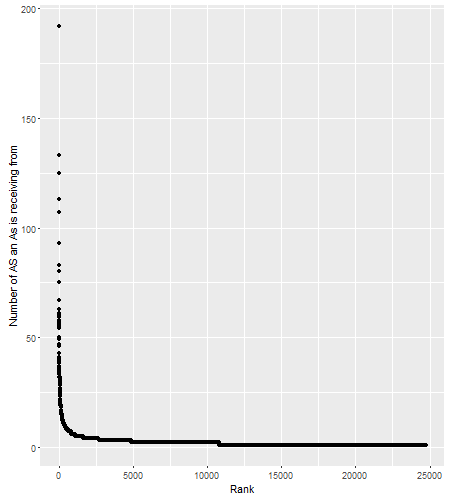
\includegraphics[scale=0.4]{Graphics/AsToDistribution.png}}
\caption{Distribution of Incoming Connections per AS}
\label{fig}
\end{figure}


Geographical Locations of ASes
\section{\\Geographical Locations of ASes}
\begin{figure}[htbp]
\centerline{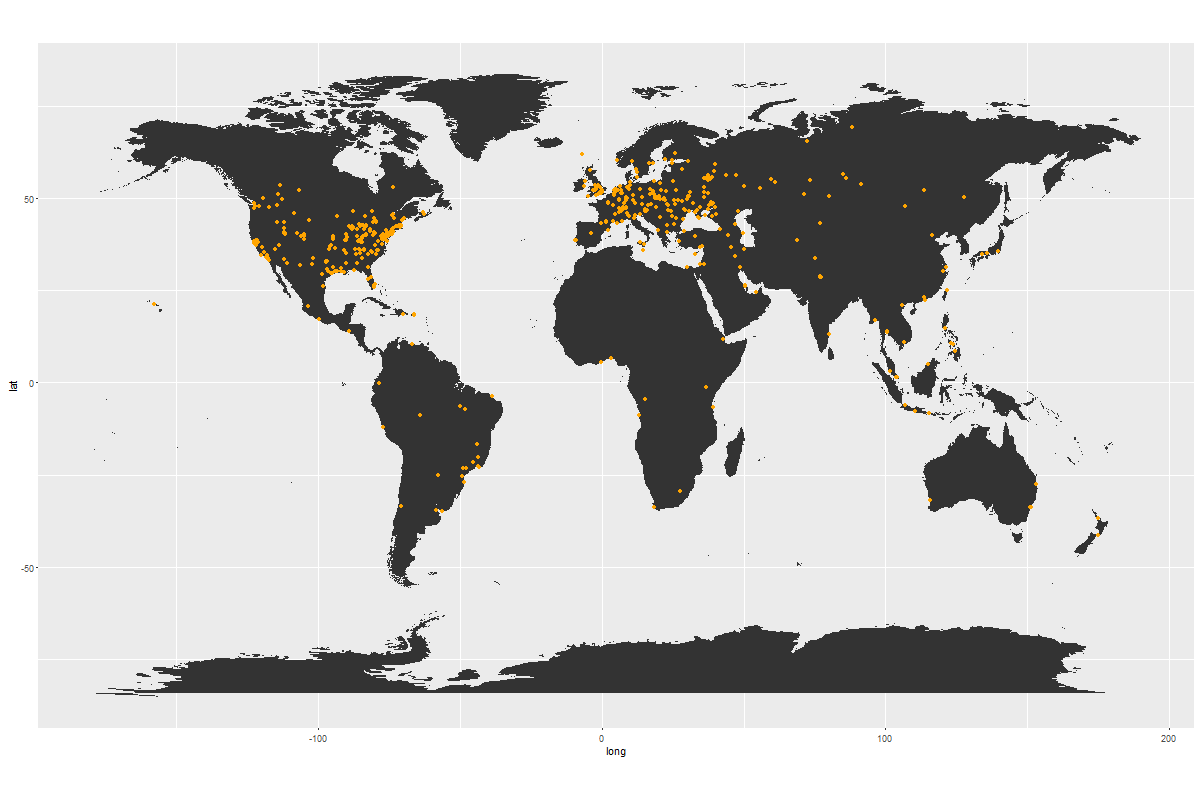
\includegraphics[scale=0.2]{Graphics/ASesNurPunkte.png}}
\caption{Geographical Locations of ASes}
\label{fig}
\end{figure}


Time development from 2007 - 2017: Number of receiving AS nodes

\begin{figure}[htbp]
\centerline{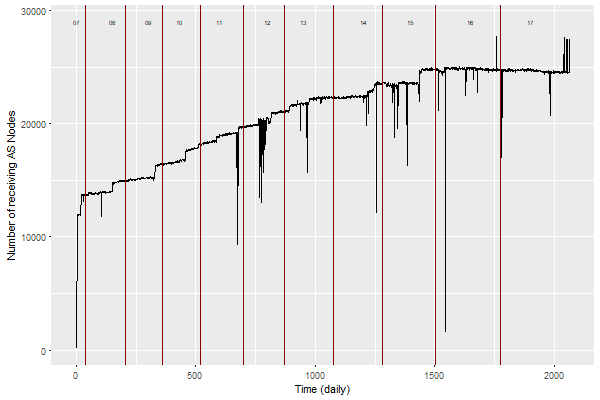
\includegraphics[scale=0.4]{Graphics/ASToAll.png}}
\caption{Time development from 2007 - 2017: Number of receiving AS nodes}
\label{fig}
\end{figure}




\section{\\Data Collection Process of CAIDA}
Data Collection Process of CAIDA





\end{document}
